\chapter{Induktionsbeviser}

Induktionsbeviser er en type beviser som typisk er nyttig til at vise diskrete sammenhænge.
Det kan eksempelvis være sætninger om naturlige tal, algoritmer eller grafer.

\begin{theorembox}{Princippet om matematisk induktion}
	De to følgende skridt skal gennemføres for at bevise at $P(n)$ er sand for alle $n \in \N$, hvor $P$ er en propositionel funktion.

	\textbf{Basisskridtet:} \quad 
	Vis $P(1)$ er sand.
	
	\textbf{Induktionsskridtet:} \quad 
	Vis at hvis $P(k)$ er sand, så følger det at $P(k + 1)$ er sand, for et vilkårligt $k \in \N$.
	Altså vis at $P \left( k \right) \to P \left( k + 1 \right)$.
\end{theorembox}

I induktionsskridtet antages det at $P(k)$ er sand for et vilkårligt $k$.
Denne antagelse kaldet induktionshypotesen.
Det kan her umildbart ligne et "cirkelbevis", fordi der antages hvad det er målet i sidste ende at vise.
Der er dog forskel på at antage en sætning for at vise denne, og at antage en sætning for at vise en anden følger heraf.
Induktionsteknikken kan skrives med formel logik som
\begin{align*}
	(P(1) \land \forall k ( P(k) \to P(k + 1))) \to \forall n P(n),
\end{align*}
hvor $n, k \in \N$. En intuitiv måde at betragte induktionsteknikken er ved at tænkte på en række af dominobrikker.
Hvis den første brik væltes, og det er sikkert at hvis en vilkårlig af brikkerne vælter, så vælter den næste også, så er må det være sandt at hele rækken vælter.
Induktionsskridtet kan altså betragtes som "dominoeffekten".
Desuden kan er det også nemt at forestille sig at hvis rækken af dominoer var uendilig lang, så vil en vilkårlig brik i rækken blive væltet hvis den første væltes. 

Induktionsbeviser kan blandt andet bruges til at bevise sætninger om summmer på de naturlige tal.
\begin{exmp}
	Vis med induktion at $1 + 3 + 5 + \dotsb + (2n-1) = n^2$, for alle $n \in \N$.

	Lad propositionen $P(n)$ være at $1 + 3 + 5 + \dotsb + (2n-1) = n^2$.
	
	\textit{Basisskridt:} $P(1)$ er sand, både da $1^2 = 1$ og summen når $n = 1$ er lig $1$.

	\textit{Induktionsskridt:} Antag at $P(k)$ er sand, for et vilkårligt $k \in \N$, Altså at $1 + 3 + 5 + \dotsb + (2k-1) = k^2$.
	Det skal nu vises at det følger at $P(k + 1)$ da også må være sand, altså at $1 + 3 + 5 + \dotsb + (2k+1) = \left( k + 1 \right) ^2$.
	\begin{align}
		&&1 + 3 + 5 + \dotsb + (2k-1) 
		&= k^2 \nonumber \\
		&\Rightarrow \quad
		&1 + 3 + 5 + \dotsb + (2k-1) + (2k+1) 
		&= k^2 + (2k + 1) \nonumber \\
		&&&= k^2 + 2k + 1 \nonumber \\
		&&&= \left( k + 1 \right) ^2 \label{eq:eks1_indu}
	\end{align}
	Her ses at $P(k + 1)$ netop er ligning \eqref{eq:eks1_indu}, hvilket betyder at $P(k + 1)$ er sand når $P(k)$ er, hvilket afslutter induktionsskridtet.

	Da både basisskridtet og induktionsskridtet er gennemført må det betyde at $1 + 3 + 5 + \dotsb + (2n-1) = n^2$, for alle $n \in \N$.
\end{exmp}

\begin{wrapfigure}{r}{5cm}
	\begin{center}
		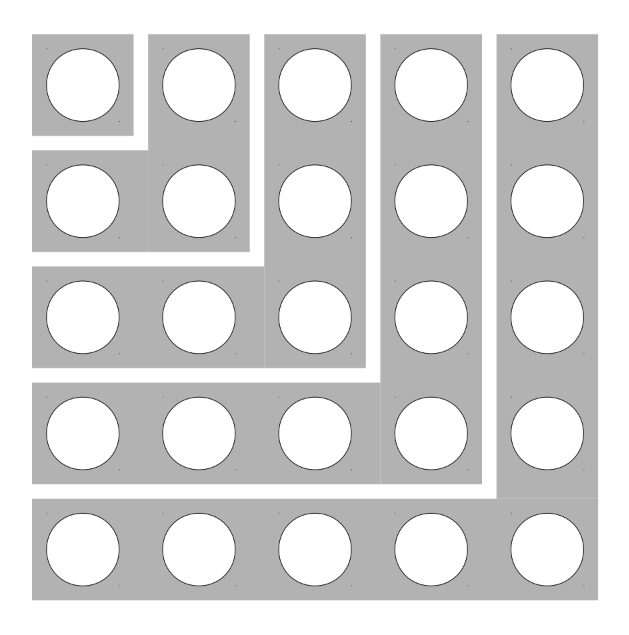
\includegraphics[scale=0.2]{fig/img/sum_of_n_first_odd_integers.png}
	\end{center}
	\caption{Bla} \label{fig1_indu}
\end{wrapfigure}

Induktionsbeviser er meget stærke, men adskiller sig fra andre bevistyper som direkte beviser, modstridsbeviser eller modeksempler ved at selve beviset ummildbart ikke skaber større forståelse for \textit{hvorfor} sætningen er sand, på samme måde som de andre måske kan gøre.

I eksempel 4.1 blev det vist at summen på de første $n$ ulige naturlige tal er lig $n^2$, men selve beviset bragte ikke større indsigt i hvorfor denne sammenhæng er sand.
Et eksempel på en indsigt om denne sammenhæng kan være figuren her (figur \ref{fig1_indu}).
Denne figur viser hvordan man altid kan arrangere summen af de første $n$ ulige tal i et kvardrat, og denne simple figur kan være del af et direkte bevis for sætningen.
Dette bevis vil meget bedre kunne illustrere sammenhængen, end det tideligere induktionsbevis.

\section{Velordensprincippet}
Induktionsbeviset bygger på en fundemental egentskab ved de naturlige tal kaldet velordensprincippet.
Det er et aktiom for de naturlige tal, og er beskrevet som følgende.
\begin{theorembox}{Velordensprincippet}
	Enhver delmængde af $\N$, der ikke er tom, har et mindste element.
\end{theorembox}
\noindent Som resultat af velordensprincippet følger det også at alle delmængder af de naturlige tal har en rækkefølge fra det mindste element, til det største, og at "det næste element i rækken" er veldifineret, da det netop det element der er det mindste i mængden foruden alle de foregående elementer.

Velordensprincippet gør det muligt at bevise induktionsbeviset er gyldig.
\begin{proof}
	Antag $P(1)$ er sand, og at $P(k) \to P(k + 1)$ er sand for alle $k \in \N$.
	Det skal nu vises at $P(n)$ da også må være sand for alle $n \in \N$.

	Antag for modstrid at $P(n)$ er falsk for mindst ét $n$.
	Lad mængden $S$ være mængden af alle $n$ hvor $P(n)$ er falsk.
	$S \subseteq \N$ må da ikke være tomt, og på grund af velordensprincippet have et mindste element $s$.
	Lad mængden $T \subseteq \N$ bestå af alle tal mindre end $s$. $s \neq 1$ da $P(1)$ er sand, hvilket betyder at $T$ ikke er tomt.
	Siden $s$ er det mindste element i $S$, må $P(t)$ være sand for alle $t \in T$, og $s - 1$ må da være et element i $T$.
	Da er $P(s-1)$ sand, og siden $P(k) \to P(k+1)$ er sand, må $P(s)$ da også være sand.
	At $P(s)$ både er sand og falsk er en modstrid.

	Da må det gælde at $(P(1) \land \forall k ( P(k) \to P(k + 1))) \to \forall n P(n)$, hvilket betyder at induktionsbeviset er gyldigt.
\end{proof}

